%!TEX root = ../../master.tex
\section{Towards a Definition}\label{sec_resilience_definitions}
The term resilience is used in several different sciences e.g. material science, engineering, psychology, and ecology. The Latin translation of resilience is \textit{"leap back"} or \textit{"bounce back"}. The Oxford dictionary equates resilience with toughness and elasticity, and an often used metaphor for illustration is a spring bouncing back. A spring is both tough and elastic. The opposite of resilience is brittleness and fragility. \\

\begin{definition} [Resilience (Oxford) \footnote{ \url{http://www.oxforddictionaries.com/definition/english/resilience}}]
\ \\
1. The capacity to recover quickly from difficulties; toughness \\
2. The ability of a substance or object to spring back into shape; elasticity
\end{definition}

\noindent
Occurrences force a resilient system to "bounce back". These occurrences are described in the literature with different terms such as a \textit{disturbance}, \textit{disruptions}, or \textit{perturbation} \cite[p. 13, 14, 19]{omer2013resilience}.\\

\noindent 
Narrowing the focus down to information and communication technology (ICT), multiple terms of resilience have a similar meaning, and it can be difficult to distinguish between them. The term \textit{resilience} in ICT has been described as the \textit{"ability to deliver, maintain, improve service when facing threats and evolutionary changes"} from a study on the usage of the word resilience in literature \cite[p. 27]{resist2007openworkshop}. In this case \textit{evolutionary changes} in current and future ICT is the important distinction from \textit{fault tolerance} \cite[p. 4]{strigini2012ftresilience}. Strigini points out that ICT systems are more interconnected, open, and exposed to more change than previously, which is why old methods for dependability do not work. This underpins the premise of this thesis and the need for new techniques to achieve dependability.

\begin{citat} []
\textit{While existing practices of dependable design deal reasonably well with achieving and predicting dependability in ICT systems that are relatively closed and unchanging, the tendency to making all kinds of ICT systems more interconnected, open, and able to change without new intervention by designers, is making existing techniques inadequate to deliver the same levels of dependability.} \textbf{- Strigini, 2012} \cite[p. 4-5]{strigini2012ftresilience}
\end{citat}

\noindent There are different ways of addressing the risk of faults in a system. \textit{Fault avoidance} is about lowering the probability of components having or developing faults, while \textit{fault tolerance} is functioning even though a fault occurs. Drawing a line between fault tolerance and \textit{resilience} can be hard, but fault tolerance covers e.g. a hardware component continuing to function in spite of an fault or error, whereas resilience also is about recovering fully (bouncing back) from failure. The step beyond resilience is the principle of \textit{antifragility} (Figure~\ref{fig:fault_handling_scale}) which was introduced by Taleb \cite[p. 1]{monperrus_2014_antifragility}. The idea is that a system gets stronger from errors (or faults) and learns from it. But as Monperrus points out this does not fit well with traditional dependability in software systems \cite[p. 1]{monperrus_2014_antifragility}. Steps toward antifragility are, though, being made as we will explain using an example from Netflix later in this chapter.
 
\begin{figure}
    \centering
    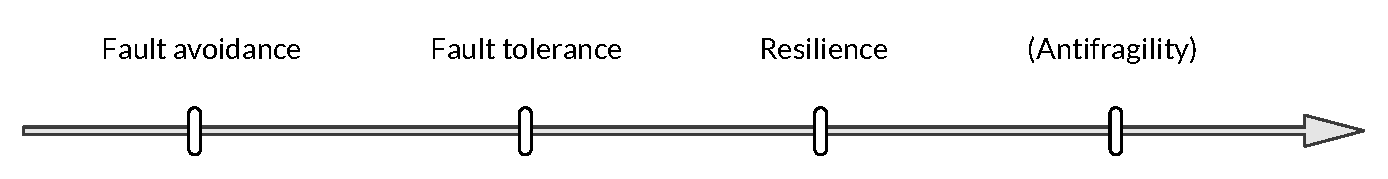
\includegraphics[width=14cm]{figures/fault_scale}
    \caption{Fault Handling Scale}
    \label{fig:fault_handling_scale}
\end{figure}